\documentclass{beamer}
\usetheme{Frankfurt}
\usepackage{color}
\usepackage{graphicx}
\usepackage[font=scriptsize,skip=1pt]{caption}
\usepackage{textpos}
\usepackage{multirow}
\usepackage{multicol}
%\usepackage{wrapfig}
\usepackage[labelformat=empty]{caption}
\usepackage[labelformat=empty,skip=0pt,justification=raggedright]{subcaption}
\usepackage{remreset}
\usepackage{multimedia}
\usepackage{mdframed}
\usepackage{natbib}
\usepackage[export]{adjustbox}

\definecolor{beaublue}{rgb}{0.74, 0.83, 0.9}
\definecolor{bubbles}{rgb}{0.91, 1.0, 1.0}
\definecolor{arsenic}{rgb}{0.23, 0.27, 0.29}
\definecolor{blizzardblue}{rgb}{0.67, 0.9, 0.93}
\definecolor{airforceblue}{rgb}{0.36, 0.54, 0.66}
\definecolor{auburn}{rgb}{0.43, 0.21, 0.1}
\definecolor{applegreen}{rgb}{0.55, 0.71, 0.0}
\definecolor{camel}{rgb}{0.76, 0.6, 0.42}
\definecolor{scarlet}{rgb}{1.0, 0.13, 0.0}
\definecolor{shamrockgreen}{rgb}{0.0, 0.62, 0.38}
\definecolor{tiffanyblue}{rgb}{0.04, 0.73, 0.71}
\definecolor{saffron}{rgb}{0.96, 0.77, 0.19}
\definecolor{aphids}{rgb}{0.85, 0.85, 0.23}
\definecolor{dummy}{rgb}{0.6, 0.6, 0.99}
\definecolor{larvae}{rgb}{0.53, 0.53, 0.21}

\setbeamercolor{section in head/foot}{fg=arsenic, bg=bubbles}
%\setbeamercolor{subsection in head/foot}{fg=black, bg=babyblue}
\setbeamercolor{frametitle}{fg=auburn, bg=white}
\setbeamercolor{upper separation line head}{bg=airforceblue}
\setbeamertemplate{section in head/foot}{\insertsectionhead}

\makeatletter
\@removefromreset{subsection}{section}
\makeatother
\setcounter{subsection}{1}


\graphicspath{{./Figures/}}

 \title{An introduction to Bayesian Data Analysis using Stan}
 \subtitle{}
 
 \author{Lionel Hertzog \& Maxime Dahirel}
 
 \date{BDA workshop, Ecology Across Border meeting\\ 13th December 2017, Gent}
 
 


\begin{document}
 
 \frame{\titlepage}
 

\begin{frame}
 \frametitle{\bf Structure of the workshop}
  \begin{enumerate}
   \item General introduction to Bayesian Data Analysis (circa. 30min)
   \item Examples of BDA workflow (circa. 30min)
   \item Small group discussion on specific themes (circa. 30min)
  \end{enumerate}
  
  Make sure to check the github page of the workshop: \url{https://github.com/lionel68/Stan-BES-2017}

 
 \end{frame}
 
\begin{frame}
 \frametitle{\bf Structure of the talk}
  \begin{itemize}
   \item What is Bayesian Data Analysis?
   \item How to do Bayesian Data Analysis?
   \item Why do Bayesian Data Analysis?
  \end{itemize}

 
 \end{frame} 
 
 
\section*{What?} 
 
 \begin{frame}
  \frametitle{\bf Why do we do Stats?}

  \begin{enumerate}
   \item To test hypothesis?
   \item To explore patterns and relationships?
   \item To predict / forecast to new place and time?
  \end{enumerate}

  \vspace*{0.5cm}

  More reasons to do stats?
  
  \vspace*{0.2cm}
  
  Bayesian data analysis is one way to do stats, it is well suited for some situation but poorly suited for others.
  
  \note{Some elements of inference, how does it fits into the science workflow
  Scientists are interested with understanding and explaining the processes structuring the world, build theories to synthetically represent what is happening.
  Data are then assembled/collected and one wants to extract the big world signal in the data, statistical inference provide this bridge between complex data and
  theories.} 
  
  
  
 \end{frame}

 
 \begin{frame}
  \frametitle{\bf Bayesians can't walk on water}

 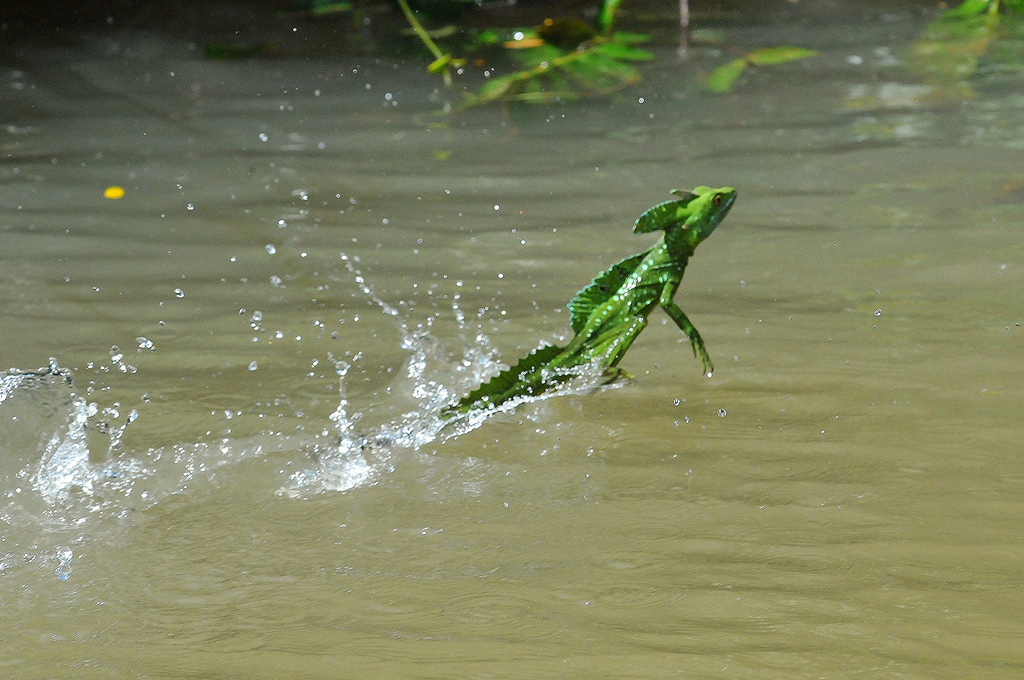
\includegraphics[width=\linewidth,height=\textheight,keepaspectratio]{water.jpg}
 
 Except maybe shallow water
\note{
  Bayesian approach cannot solve experimental design issue, e.g. wanting to find effect of competition with N=2 ...
}
  
 \end{frame}
 
 \begin{frame}
  \frametitle{\bf There is no bayesian model}
  
  \begin{figure}
    
\includegraphics[width=\textwidth,height=.8\textheight,keepaspectratio]{bayes_model.jpg}
  \end{figure}

 
  

   \note{Bayesian data analaysis uses the same models as developed in classical stats,
   so there is no hierarchical bayesian models, but rather hierarchical models fit using a
   bayesian framework, this is pretty comforting as this means that we can continue fitting the same
   model we've been using except this time with all advantages confered by bayesian data analysis.}

  
 \end{frame}
 
  \begin{frame}
  \frametitle{\bf What is Bayesian Data Analysis?}
  
    
  $Posterior \propto Likelihood * Prior$
  
  \vspace*{1cm}
  
  Or:
  
  \vspace*{1cm}
  
  New knowledge $\propto$ new data * prior knowledge
  
  \vspace*{1cm}
  
  Bayesian data analysis updates prior knowledge (or belief) based on new data.
  
 \end{frame}
 
 
 \begin{frame}
  \frametitle{\bf The Likelihood: what we've been doing all of our lives}
  
 \[
  lm(y \sim x1 + x2, data)
 \]

  
  This is equivalent to:
  
  \[
   y_i \sim \mathcal{N}(\mu_i,\, \sigma)   
   \]
   
   \[
    \mu_i = a + b_1 * x1 + b_2 * x2
   \]

Which is called the \textsc{likelihood}, the probability of the data given the model. 
   
  
  \note{Prob of the data knowing the parameters, what is hidden behind the (G)LM(M) motor
  
  Some plot of what this means  
  
  Good news is: we do not need to learn new models}
  
 \end{frame}
 
 \begin{frame}
  \frametitle{\bf The likelihood: a graphical example}
  
  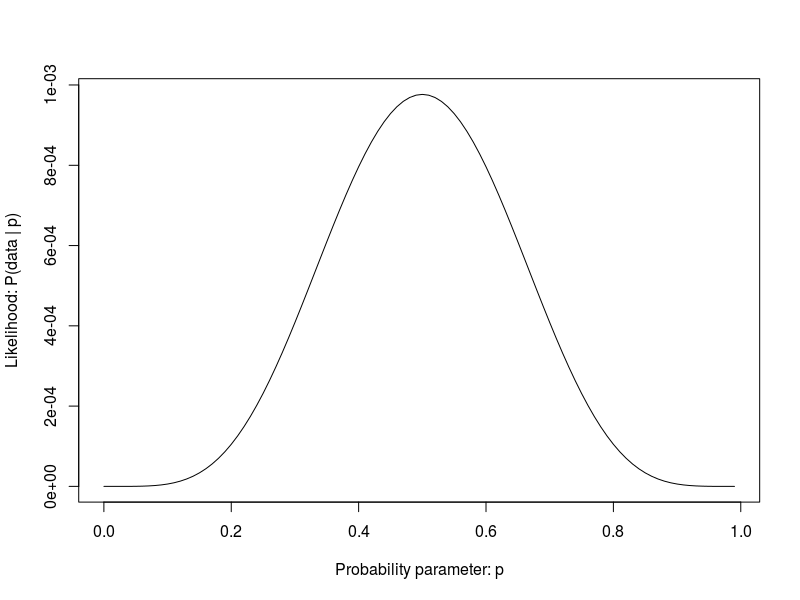
\includegraphics[width=\textwidth,height=.75\textheight,keepaspectratio]{likelihood.png}
  
  \[
   y \sim \mathcal{B}(n = 10,size = 1,prob = 0.5)
  \]
  
  \note{critical part of modelling: as long as we can write down the likelihood of our model we have great freedom}

  
 \end{frame}

 \begin{frame}
  \frametitle{\bf The prior: our eductaed guess about the world}
  
  Amongst the following probability distribution which one would you think represent plausible distribution of the slope of plant richness effect on plant biomass?
  
  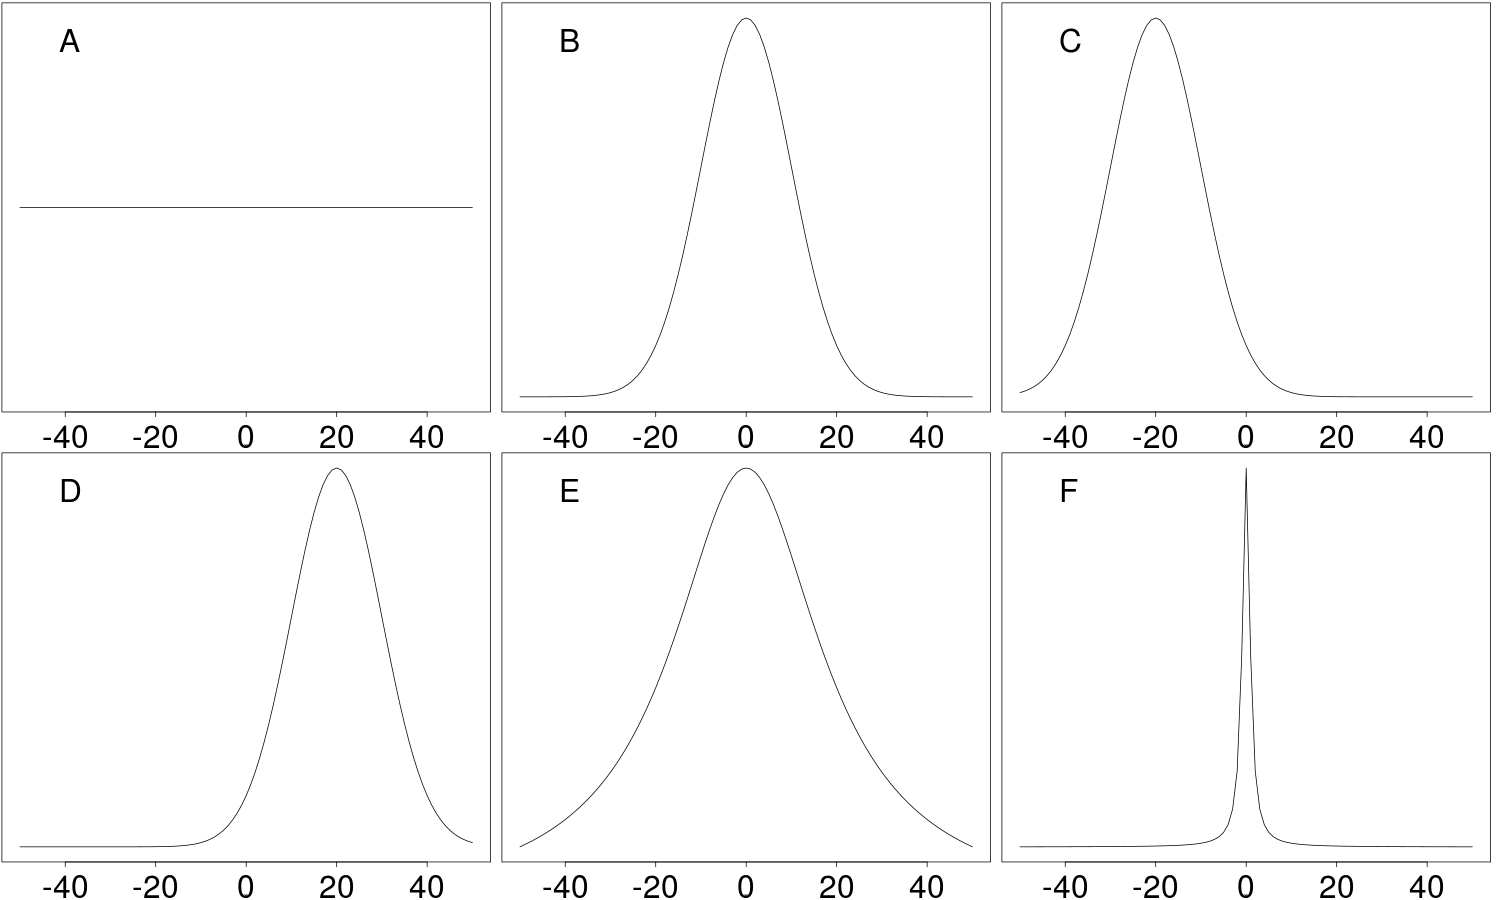
\includegraphics[width=.9\textwidth,height=.7\textheight,keepaspectratio]{prior_choice.png}
  
  \note{This is something new, prior is also a probability distribution that represent our beliefs of the likely values of the parameters
  This is the information that is around in the literature or in the community before doing an analysis
  Example: want to explore plant growth or whatever with a meta-analysis
  And/or information based on the nature of the parameter
  Example: a time parameter will likely be >= 0}
  
 \end{frame}
 
  \begin{frame}
  \frametitle{\bf The posterior: everything we ever wanted (from a statistical model)}
  
  \begin{columns}
   \column{.3\textwidth}
    \begin{itemize}
     \item Combine prior infos with new data
     \item Probability (density) of the parameter 
     \item Weight of prior decline as sample size increases
    \end{itemize}
    
    \column{.7\textwidth}
    \only<1>{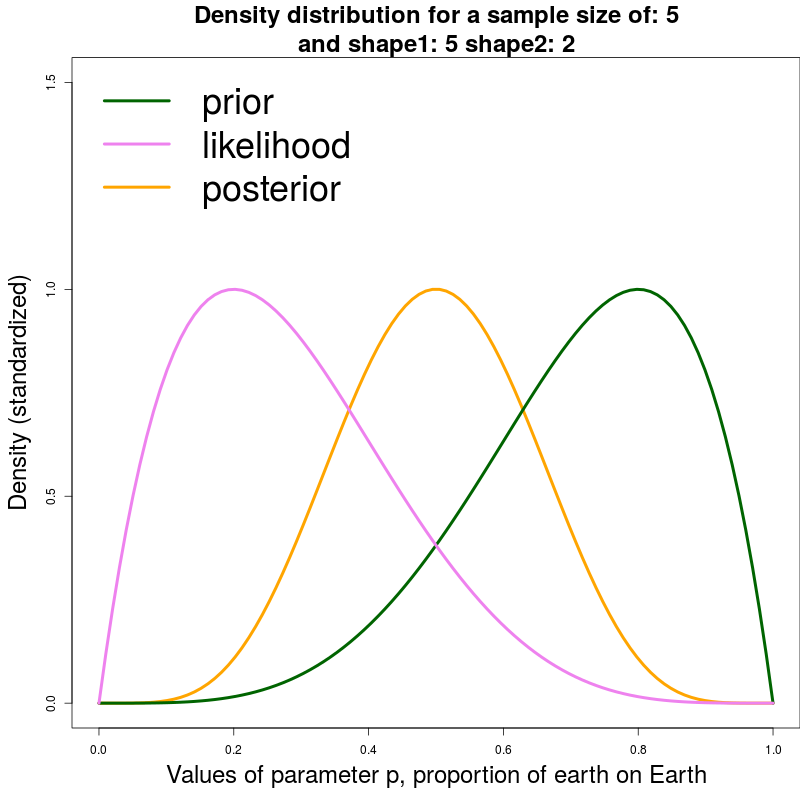
\includegraphics[width=\textwidth,height=\textheight,keepaspectratio]{post1.png}}
    \only<2>{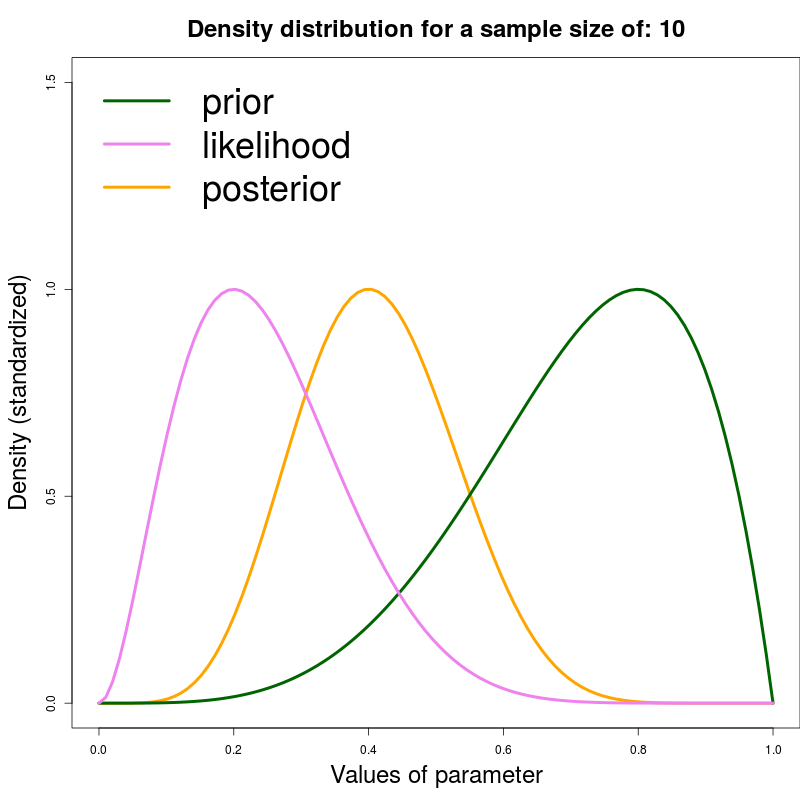
\includegraphics[width=\textwidth,height=\textheight,keepaspectratio]{post2.png}}
    \only<3>{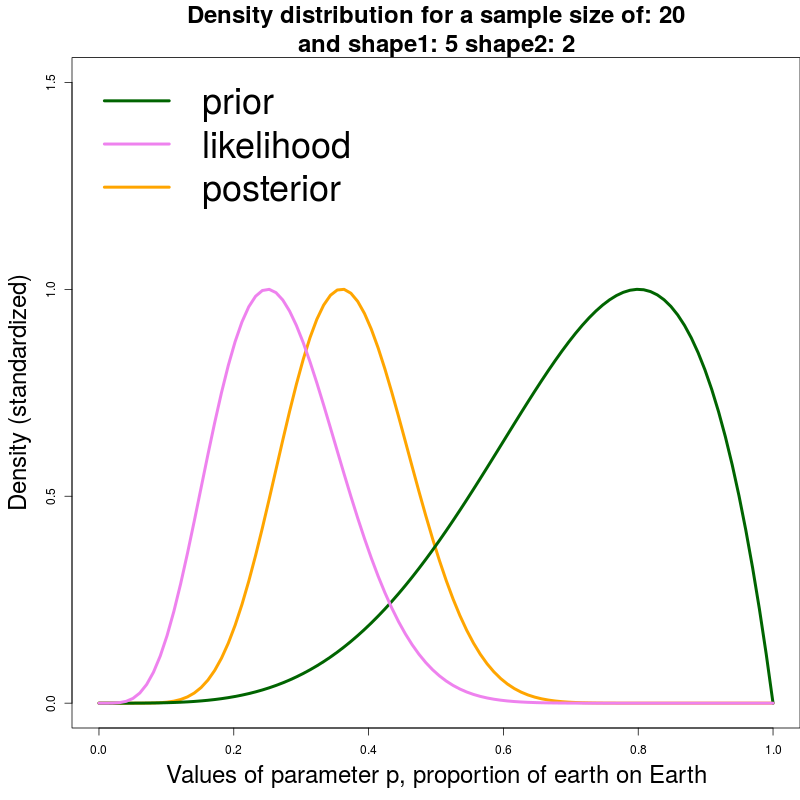
\includegraphics[width=\textwidth,height=\textheight,keepaspectratio]{post3.png}}
    \only<4>{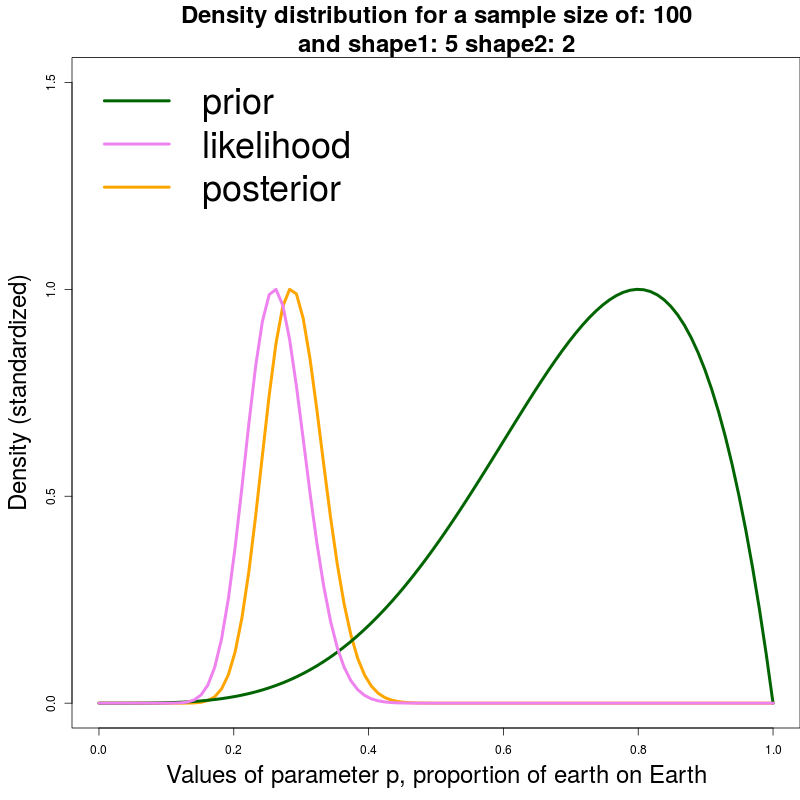
\includegraphics[width=\textwidth,height=\textheight,keepaspectratio]{post4.png}}
    \only<5>{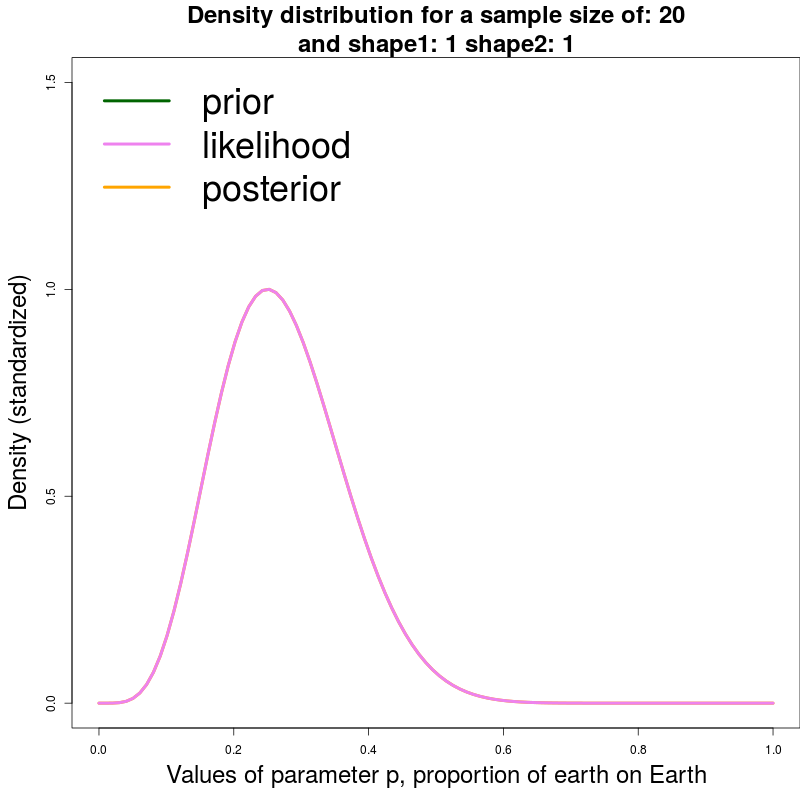
\includegraphics[width=\textwidth,height=\textheight,keepaspectratio]{post5.png}}
%\if possible adjust so that images and text don't move up and down during animations
  \end{columns}

  \note{
  
  The posterior is also a probability distribution, it quantifies the probability of parameter values knowing the data (the likelihood) and our expectation (prior)
  The impact of the data vs the expectation depends on the sample size, with low sample size the prior is relatively more important (little information in the data), as
  sample size grows the likelihood gets more and more weights, a simple example (maybe a shiny app ...)
  % I like the idea of the shiny app, maybe using a simple example like the prop water/land in the StatRethinking book?
  }
  
  \end{frame}


 
 
\begin{frame}
 \frametitle{\bf The key aspects of BDA}
 
 \begin{figure}
  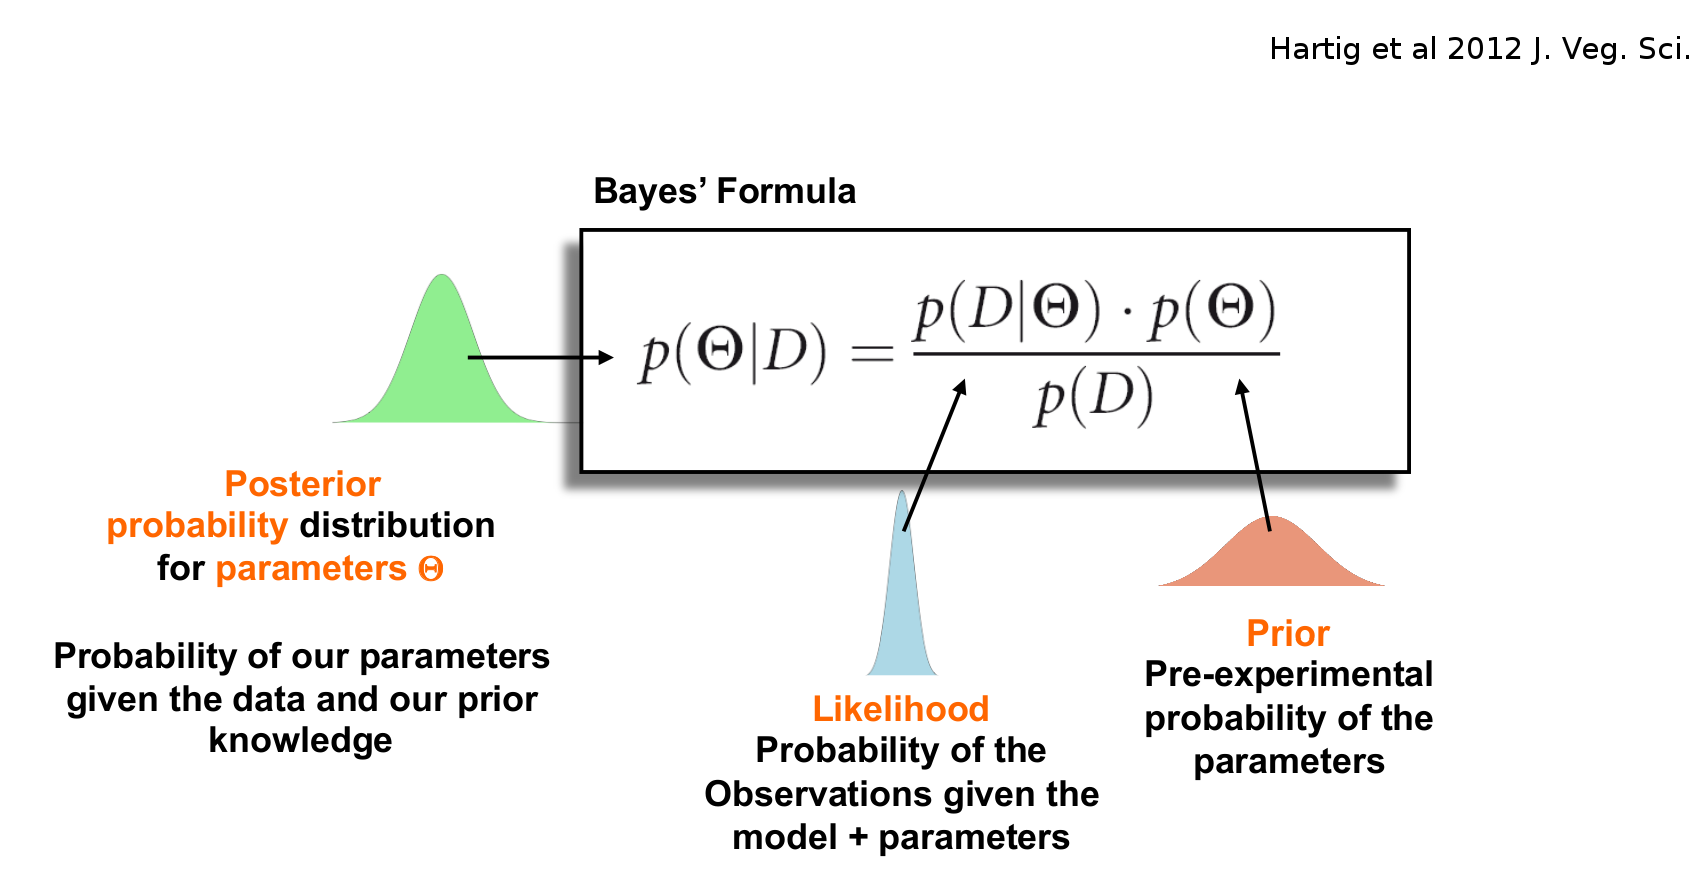
\includegraphics[width=\textwidth,height=.75\textheight,keepaspectratio]{summ.png}
 \end{figure}
 
 \begin{columns}
  \column{.45\textwidth}
   \begin{itemize}
    \item Everything is distribution
    \item Integrate prior knowledge
   \end{itemize}
   
   \column{.5\textwidth}
    \begin{itemize}
     \item Models as data-generators
     \item Easy interpretation
    \end{itemize}


 \end{columns}


 \note{
 Explicitly integrate prior knowledge 
 Output probability for the parameters/hypothesis, posterior
 Uncertainty is everywhere
 Think of models as data-generating processes}
 
\end{frame}

\section{How?}

 \begin{frame}
  \frametitle{\bf Ways to fit bayesian models in R}
  
  
  
  Two main options are available to fit bayesian models in R:
  
  \vspace{1cm}
  
  \begin{columns}
   \column{.5\textwidth}
   Directly using a dedicated probability language:
   \begin{itemize}
    \item JAGS via rjags
    \item Stan via rstan
   \end{itemize}
   
   \column{.5\textwidth}
   Using packages that translate R formulas into the probability language:
   \begin{itemize}
    \item rstanarm
    \item brms
   \end{itemize}


  \end{columns}

  
  \note{Coding in probability language vs using wrappers
  Stan is a programming language in its own so can code the models direclty in it (some snippet code example of simple model)
  Knowing this we have the full flexibility to fit any model we want but we also have the full possibility that we make coding/interpretation
  errors that are not visible.
  There are a couple of R packages to transcribe the standard R formula synthax into Stan models: rstanarm and brms. With this option we are sure that the model
  code is correct and also optimized so it will certainly run faster than naive implementation directly in Stan. But one is limited by what the package developers have
  implemented.}
  
 \end{frame}

  \begin{frame}
  \frametitle{\bf The sampling: the issue of complex likelihood surface}
  
  \note{Blind man in the likelihood landscape, how do we effectively sample it, it is hard to compute the integral in the numerator for typical analysis problems so we have to rely on computational techniques}
  
  \begin{figure}
   \only<1>{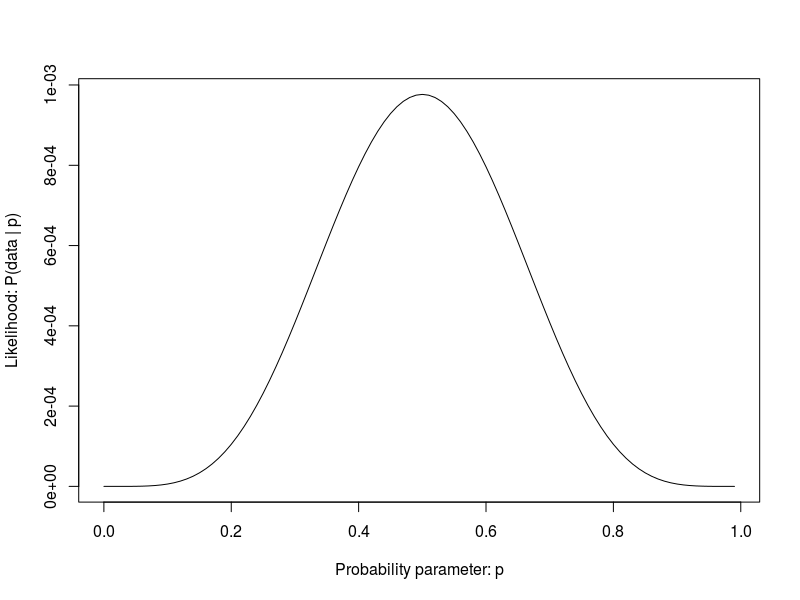
\includegraphics[width=\textwidth,height=.7\textheight,keepaspectratio]{likelihood.png}}
   \only<2>{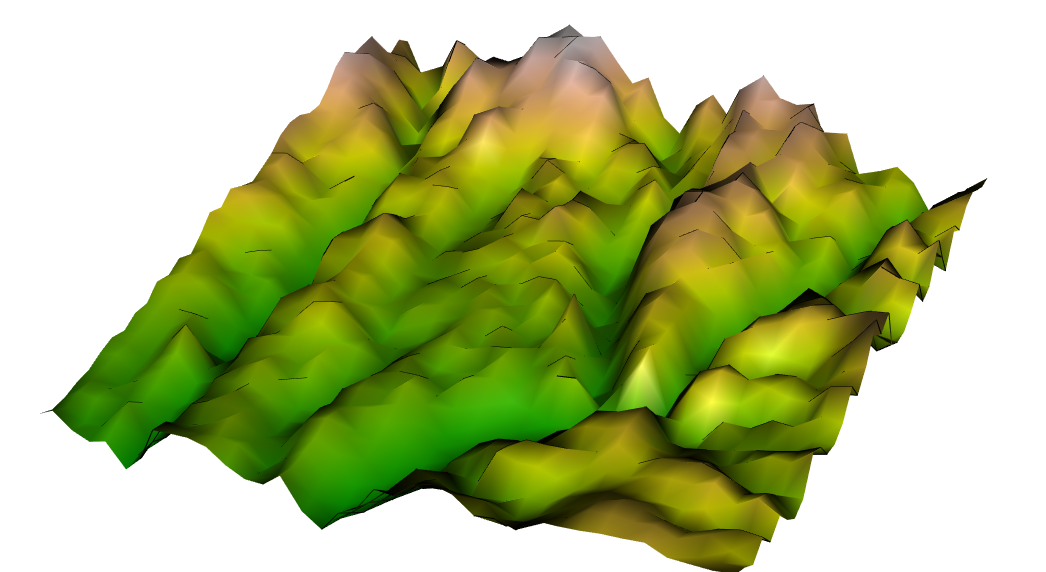
\includegraphics[width=\textwidth,height=.7\textheight,keepaspectratio]{like_surf.png}}
  \end{figure}

  \only<2>{\scriptsize The sampler should travel around in the likelihood space but spend more time in area of high likelihood mass than in area of low likelihood mass}
  %\maybe add an animation showing the first likelihood plot from a few slides before first, so that people better understand what this one is
  
  
 \end{frame}
 
 \begin{frame}
  \frametitle{\bf A simple Markov Chain Monte Carlo algorithm}
  
  \begin{enumerate}
   \item Start with arbitrary parameter values and compute the posterior (likelihood times prior) at this point
   \item Pick new values for all parameter in the model (based on some proposal distribution)
   \item Compute the new posterior for these values
   \item If the new posterior is larger than the old one, accept the new value (take one sample) if not jump to the new value based on some probability
  \end{enumerate}

  See: \url{https://theoreticalecology.wordpress.com/2010/09/17/metropolis-hastings-mcmc-in-r/} 
  
  \note{Markov Chain Monte Carlo: stochastic transition within parameter space only based on current and proposed jump.
  Key point: at convergence the MCMC samples will equal the posterior distribution, the MCMC samples are not stricto sensu the posterior}
  
 \end{frame}
 
 \begin{frame}
  \frametitle{\bf A simple MCMC example: How much earth is on Earth?}
  
  \begin{columns}
   \column{.4\textwidth}
    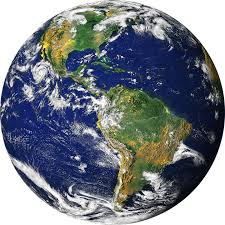
\includegraphics[width=\textwidth,height=.4\textheight,keepaspectratio]{globe.jpeg}
    
    \only<1>{We tossed the globe 10 times and we landed 3 times on land. The parameter to estimate is: $\mathcal{B}(10, p)$, we assume flat prior.
    
    \vspace*{0.1cm}
    
    {\tiny (Example from Statistical rethinking, Richard McElreath)}}
    
    \only<2->{
    
    \vspace*{0.5cm}
    
    MCMC samples:}
    
    \vspace*{0.3cm}
    
    \only<2->{0.5}\only<4->{, 0.2}
    
    
   \column{.6\textwidth}    
   
   \only<1>{
   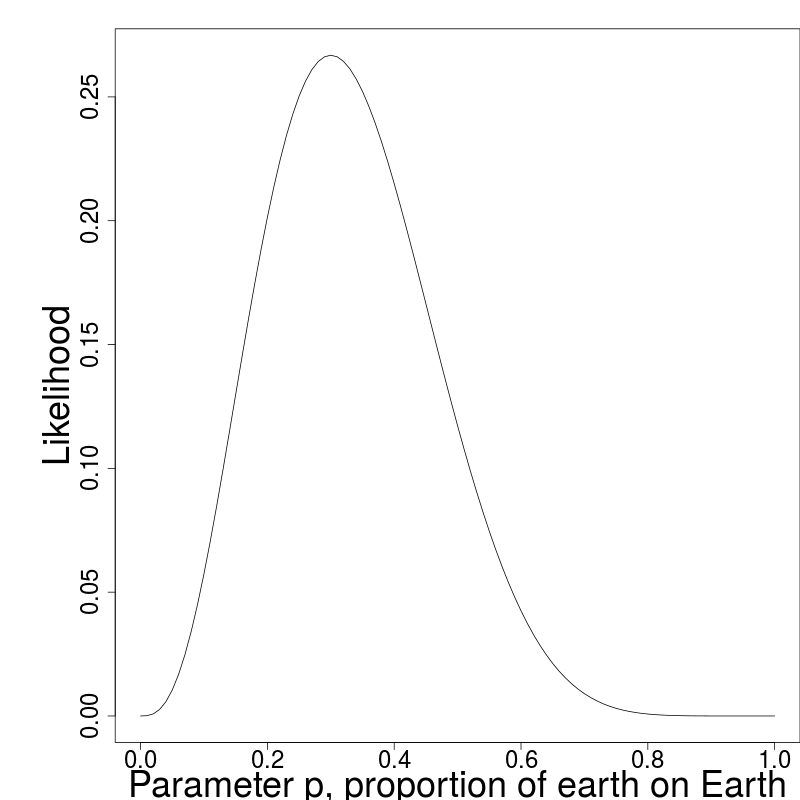
\includegraphics[width=\textwidth,height=.7\textheight]{Likelihood_start.png}
   
   \vspace*{0.5cm}
   
   }
   
      \only<2>{\scriptsize
      
       Pick a starting value: 0.5, the likelihood is: 0.12
       
       \vspace*{0.3cm}
      
   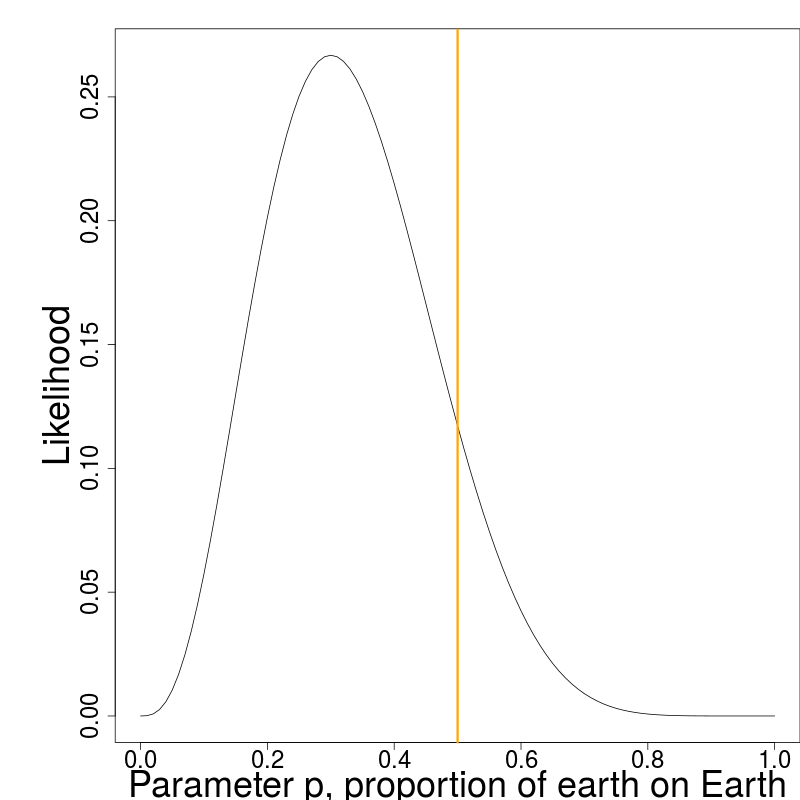
\includegraphics[width=\textwidth,height=.7\textheight]{Likelihood_init.png}   
   }
   
         \only<3>{\scriptsize
         
         Pick a new value: 0.2, the new likelihood is: 0.20
         
         \vspace*{0.3cm}
         
   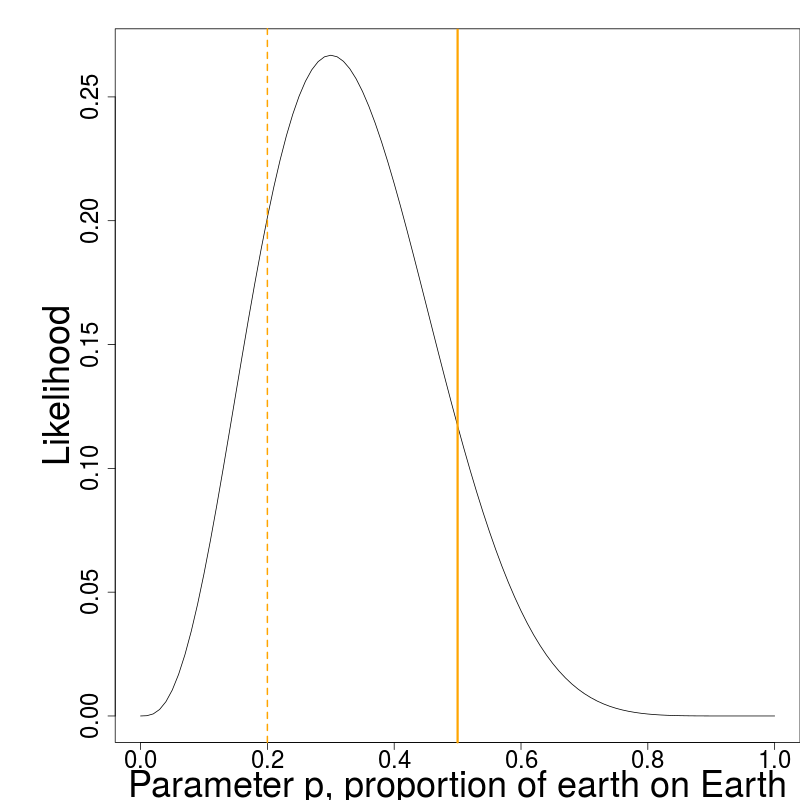
\includegraphics[width=\textwidth,height=.7\textheight]{Likelihood_1.png}   
   }
   
         \only<4>{\scriptsize
         
         Old likelihood \textless~New likelihood, jump.
         
          \vspace*{0.3cm}
         
   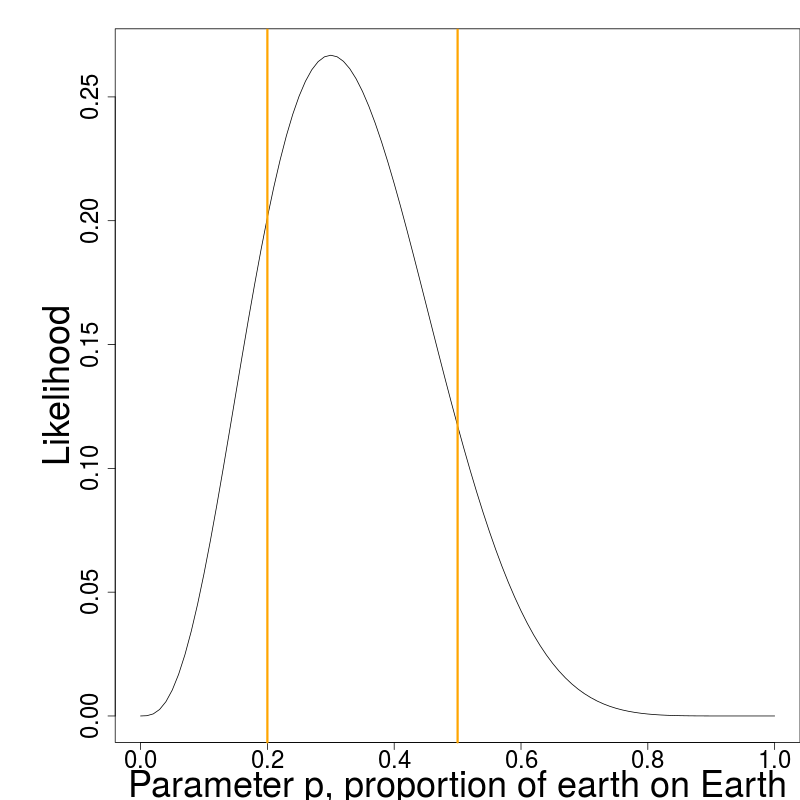
\includegraphics[width=\textwidth,height=.7\textheight]{Likelihood_2.png}     
   }
   
            \only<5>{\scriptsize
         
        Pick a new value: 0.15, the new likelihood is: 0.13
         
          \vspace*{0.3cm}
         
   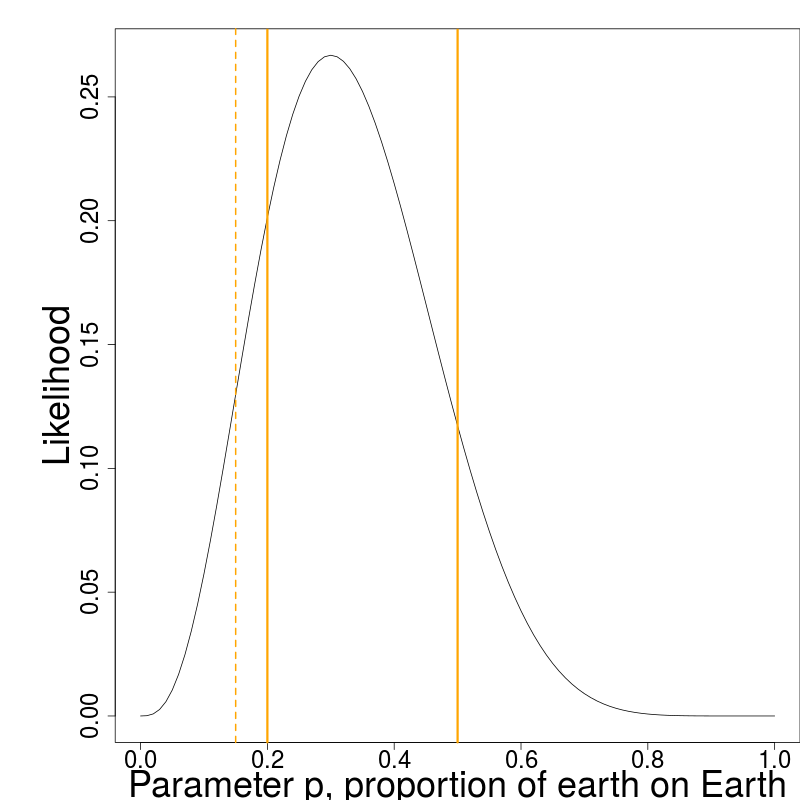
\includegraphics[width=\textwidth,height=.7\textheight]{Likelihood_3.png}     
   }
   
               \only<6>{\scriptsize
         
        The new value will be accepted with a probability of 0.13 / 0.20
         
          \vspace*{0.3cm}
         
   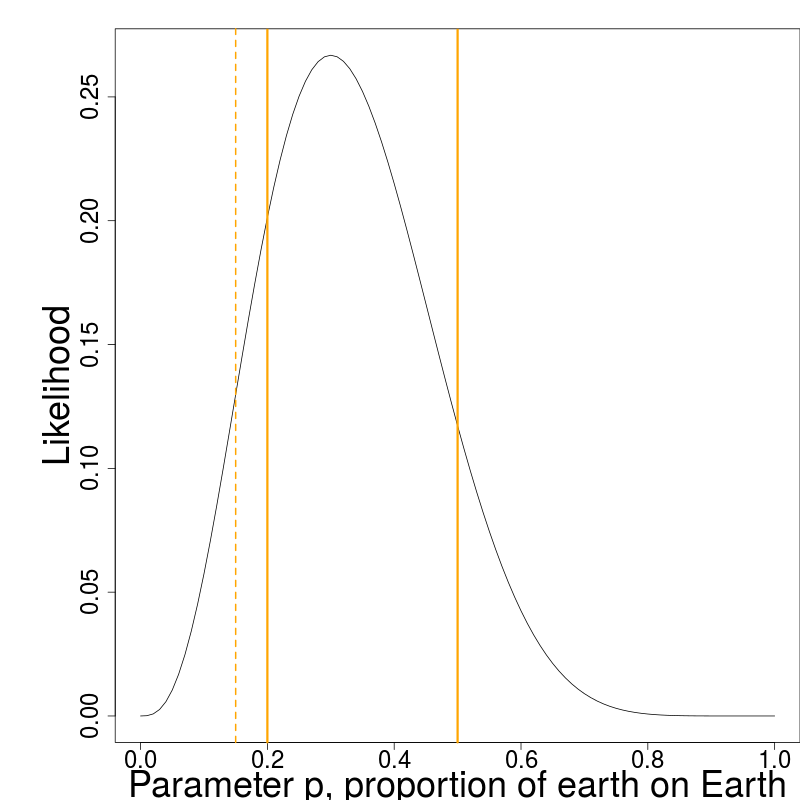
\includegraphics[width=\textwidth,height=.7\textheight]{Likelihood_3.png}     
   }
   
                  \only<7>{\scriptsize
         
        The jump failed, go back to previous value
         
          \vspace*{0.3cm}
         
   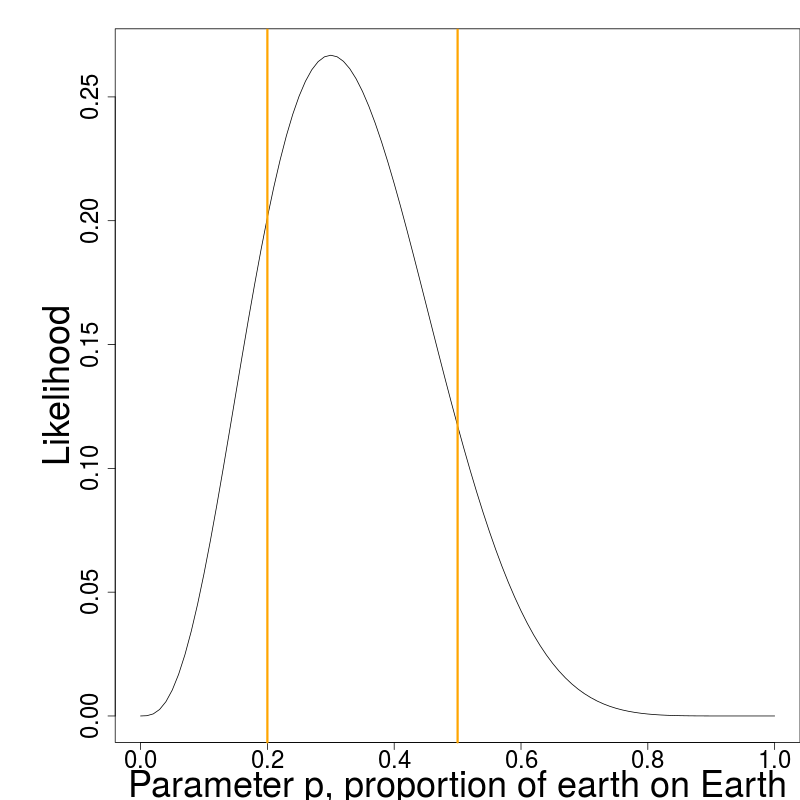
\includegraphics[width=\textwidth,height=.7\textheight]{Likelihood_2.png}     
   }
   
   \only<8>{
    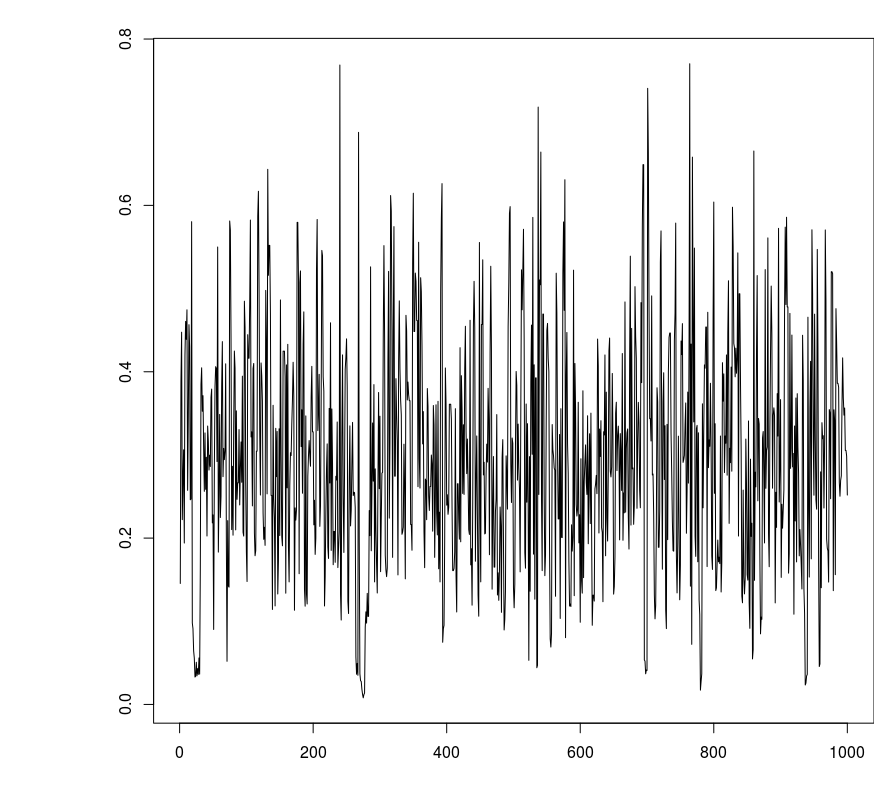
\includegraphics[width=\textwidth,height=\textheight,keepaspectratio]{trace.png}
   }
             
  %\if possible adjust so that images and text don't move up and down during animations 
   
     
    \note{\only<2->{We pick a starting value of 0.5, the likelihood at this starting value is: 0.12} 
    
    \vspace*{0.1cm}
    
    \only<3->{From our prior we pick a new parameter value of 0.2, the likelihood there is: 0.20} 
    
    \vspace*{0.1cm}
    
    \only<4->{The sampler jump to this new value; we pick a new value (0.15), the likelihood there is: 0.13} 
    
    \vspace*{0.1cm}
    
    \only<5->{We compute the ratio of new to old likelihood (0.65), this is the probability that the sampler jump to this value}
    
    \vspace*{0.1cm}
    
    \only<6->{The jump failed, the sampler stay at the old value (0.2) and a new valus is picked} 
    
    \vspace*{0.1cm}
    
    \only<7>{Do this many times}}
   
  \end{columns}

  
  
  
  
  
 \end{frame}



  \begin{frame}
  \frametitle{\bf Different MCMC algorithm / samplers}
  
  Different MCMC algorithms are available:
  
  \begin{itemize}
   \item JAGS: uses (mainly) Gibbs sampling which in essence decompose a complex problem into a set of simple ones, if possible JAGS will automatically sample from the posterior (conjugacy)
   \item Stan: uses Hamiltonian-Monte Carlo, it gives momentum and gravity to the sampler, it is more efficient for sampling the posterior (fewer samples needed)
  \end{itemize}
  
  For more infos see:\\
  M. Betancourt, \url{https://arxiv.org/abs/1701.02434}\\
  C.C. Monnahan, \url{http://onlinelibrary.wiley.com/doi/10.1111/2041-210X.12681/full}\\
  \url{https://www.youtube.com/watch?v=VnNdhsm0rJQ}
  
 \end{frame}
 
   
  \begin{frame}
  \frametitle{\bf Elements of Bayesian vocabulary}
  
   \begin{itemize}
   \item Chains: number of Markov chains ran, best to have at least 3
   \item Convergence: property of the Markov chains, at convergence the MCMC samples represent the posterior distribution
   \item Divergence: property of the Markov chains, when the sampler does not effectively move in the parameter space, in Stan it specifically means that the Hamiltonian dynamics ran into that indicates potential bias in estimates.
   \item Rhat: indicator to check convergence of the Markov chains, a value of 1 indicate convergence
   \item n\_eff: number of effective samples, due to autocorrelation in the Markov chains fewer samples are taken than expected, n\_eff / number of MCMC samples should be larger than 0.1
  \end{itemize}

  
 \end{frame}
 
  \begin{frame}
  \frametitle{\bf Model checking in Bayesian data analysis}
  
  Your best friend for model checking is the \textbf{shinystan} package
  
  \begin{figure}
   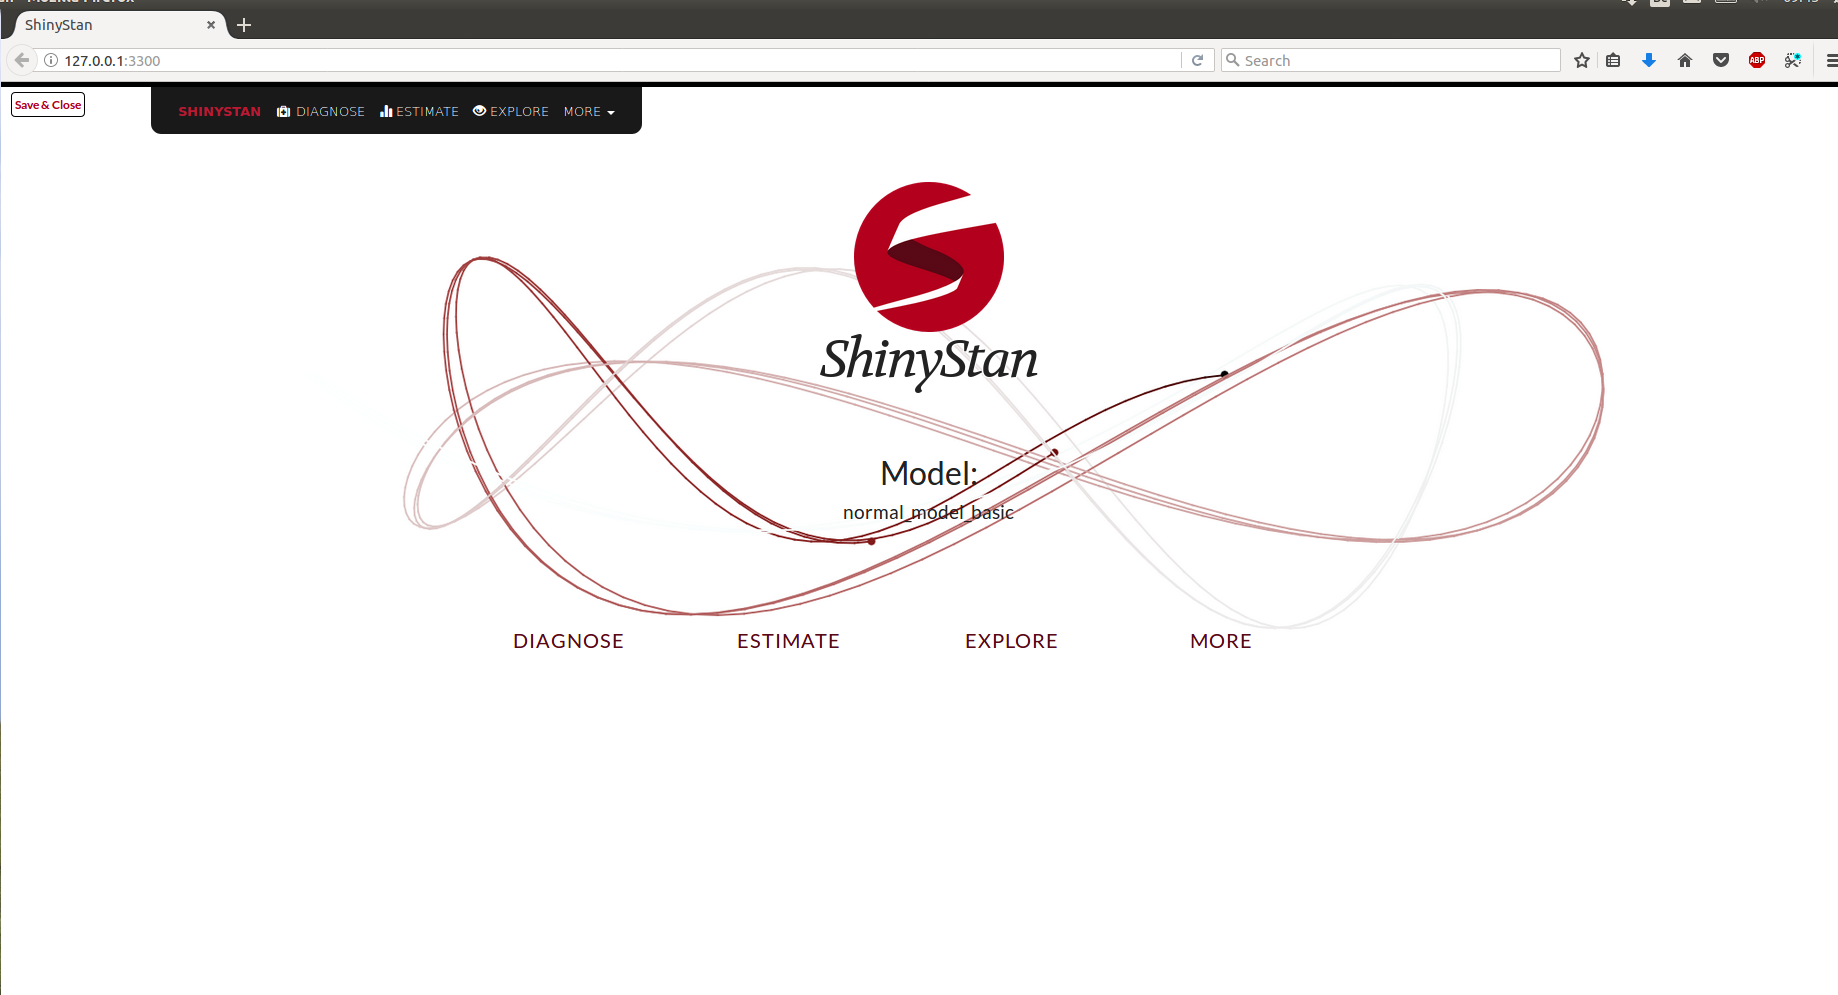
\includegraphics[width=\textwidth,height=.7\textheight,keepaspectratio]{shiny.png}
  \end{figure}
  
  To be explored during the coding session

  
 \end{frame}
 
  \begin{frame}
  \frametitle{\bf Model comparison/selection}
  
  A couple of information criteria metrics should be used:
  
  \begin{enumerate}
   \item Watanabe-Akaike Information Criteria: basically the summed log likelihood over the posterior samples (predictive density) minus the effective number of parameters, better than the DIC since it uses all posterior samples instead of point estimates.
   \item Leave-One Out cross-validation: drop one data point at a time and re-estimate the predictive density, this methods is commonly used for machine learning models to avoid problems like overfitting.
  \end{enumerate}
  
  \vspace*{0.2cm}
  
  Both are readily available for Stan models through the \textbf{loo} package

  
 \end{frame}
 

\section{Why?}
 
  \begin{frame}
  \frametitle{\bf Embracing uncertainty}
  
  \begin{figure}
   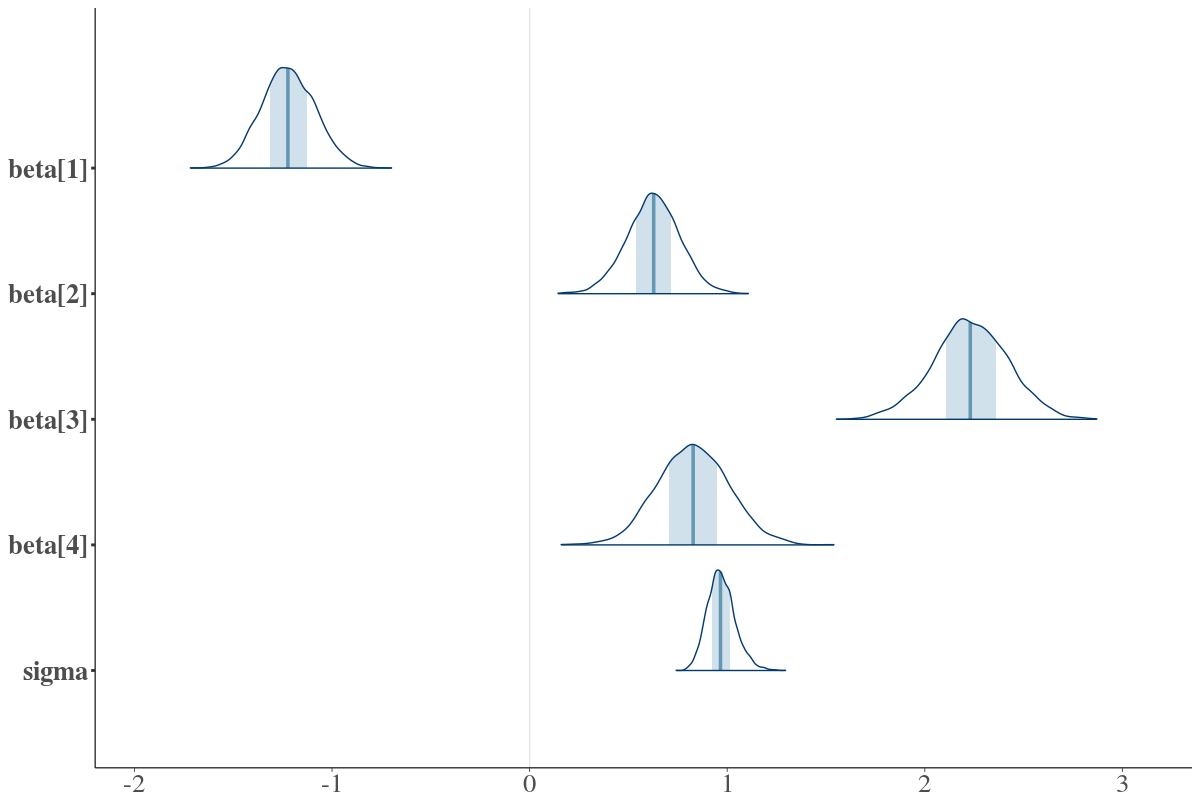
\includegraphics[width=\textwidth,height=.7\textheight,keepaspectratio]{posterior-params.png}
  \end{figure}

  
  \note{Everything is variable, all parameters come with (posterior) distribution, can interprete posterior sample
  as probabilities, flexibility to test any hypothesis building on these}
  
 \end{frame}
 
  \begin{frame}
  \frametitle{\bf Flexibility in model building}
  
  It all comes down to the likelihood, as long as you can write down the likelihood function you can fit whatever model you want.
  
  \begin{figure}
   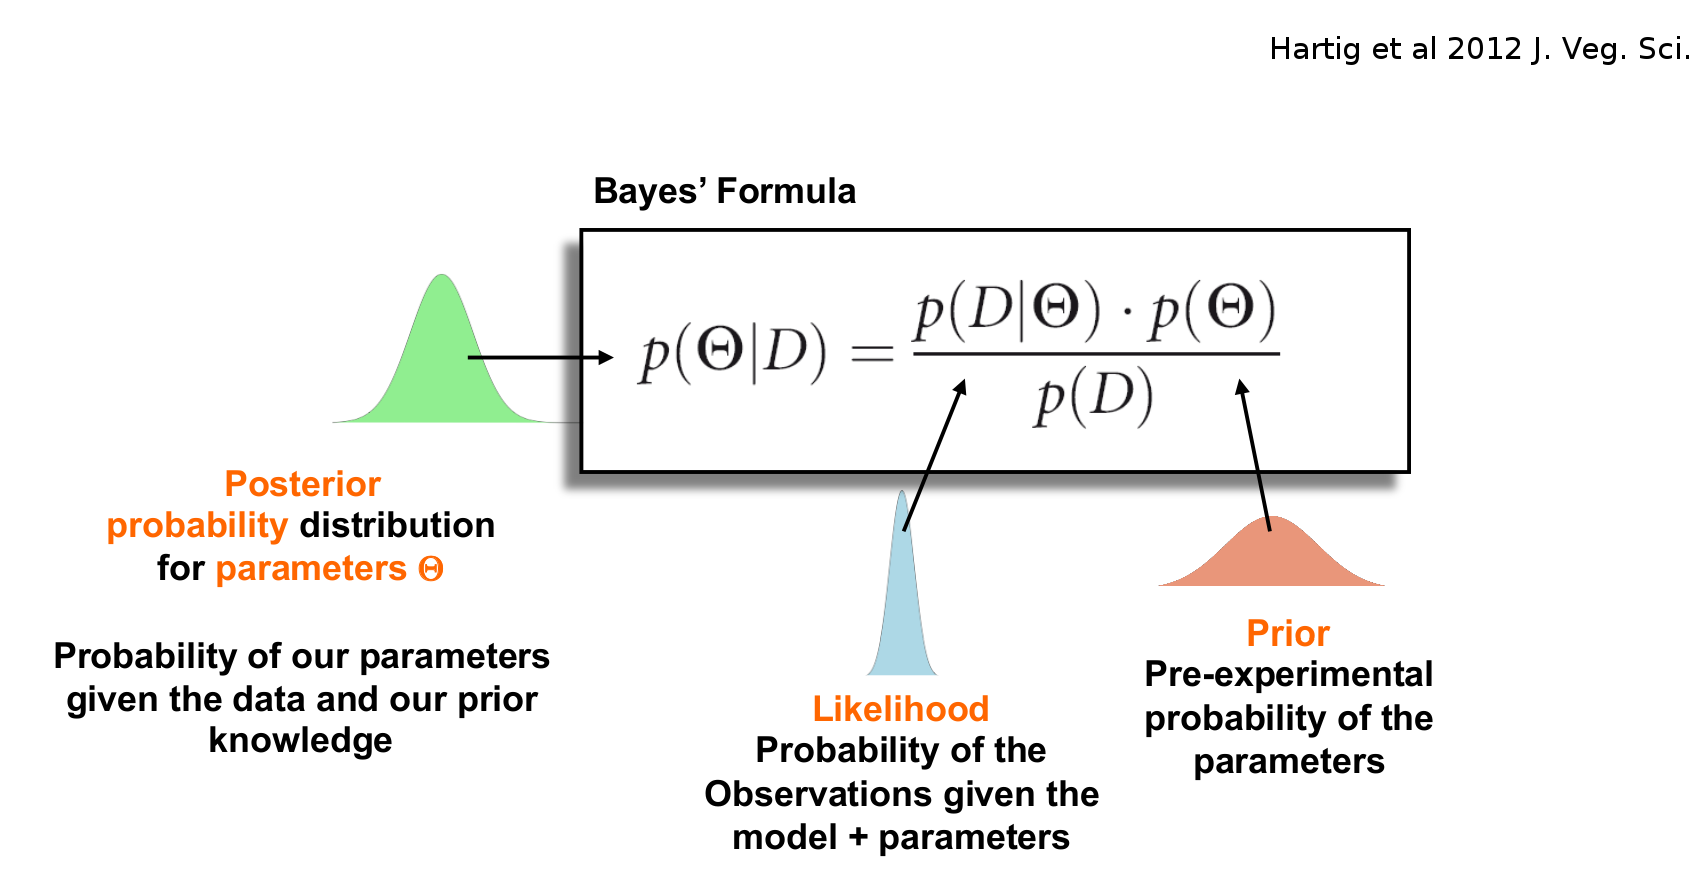
\includegraphics[width=.7\textwidth,height=.6\textheight,keepaspectratio]{summ.png}
  \end{figure}

   \note{As long as you can write your likelihood function you can fit any model you like (similar to using MLE approach
  ie with bbmle)}
  
 \end{frame}
 
 \begin{frame}
  \frametitle{\bf Models as data-generating processes}
  
  \begin{figure}
   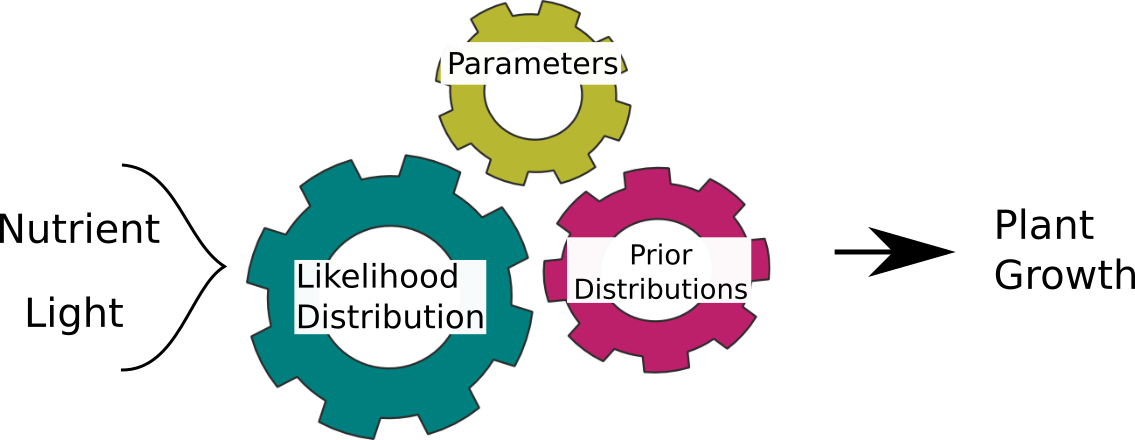
\includegraphics[width=\textwidth,height=.7\textheight,keepaspectratio]{cogs_f.png}
  \end{figure}

  Note that this also applies to frequentist approaches (assuming fixed parameter values)
  
 \end{frame}

 
  \begin{frame}
  \frametitle{\bf Bayesian approach output is what we actually want}
  
  Posterior samples from the MCMC can be interpreted as probabilities.\\
  
  \vspace*{0.3cm}
  
  It is easy and straightforward to manipulate them to get what you want (probability intervals, hypothesis tests ...) all with easy interpretation.\\
  
  \vspace*{0.3cm}
  
  Very different from complex and convoluted concepts like p-values, confidence intervals, null hypothesis ...
  
   \note{Bayesian data analysis give us relevant answers in terms of probability rather than weird answers refering to some null hypothesis in
  terms of frequency, }
  
 \end{frame}
 
  \begin{frame}
  \frametitle{\bf No degrees of freedom}
  
  With Bayesian approach we can fit models with more parameters than data points
  
  \vspace*{0.3cm}
  
  This is due to the prior distributions, it provides extra information to the model along the observed data
  
  \vspace*{0.3cm}
  
  BUT this does not absolve us from statistical machismo (sensu Brian McGill)
  
 \end{frame}
 
  \begin{frame}
  \frametitle{\bf Asymptotic convergence, when bayesian and frequentist approach give similar answers}
  
  As sample size increase the posterior is drawn closer and closer to the likelihood, in other words at infinite sample size the posterior is the likelihood
  
  \vspace*{0.3cm}
  
  The relative importance of the likelihood vs the prior depends on the complexity of the models, if sample size is fixed, the more parameters, the more the posterior is affected by the prior
  
  \note{With infinite sample size the posterior distribution just reflect the likelihood, as sample size increases
  priors have dwindling effects}
  
 \end{frame}
 
 \section*{}
 
 \begin{frame}
  \frametitle{\bf Time for some coding}
  
 \begin{center}
  Open the \textit{model\_fitting\_script.R} file
 \end{center}
 
\end{frame}
 
\end{document}


 \begin{frame}
  \frametitle{\bf }
  
 \end{frame}

